\chapter{Interfaz y Navegación Básica}

\begin{figure}[H]
	\centering
	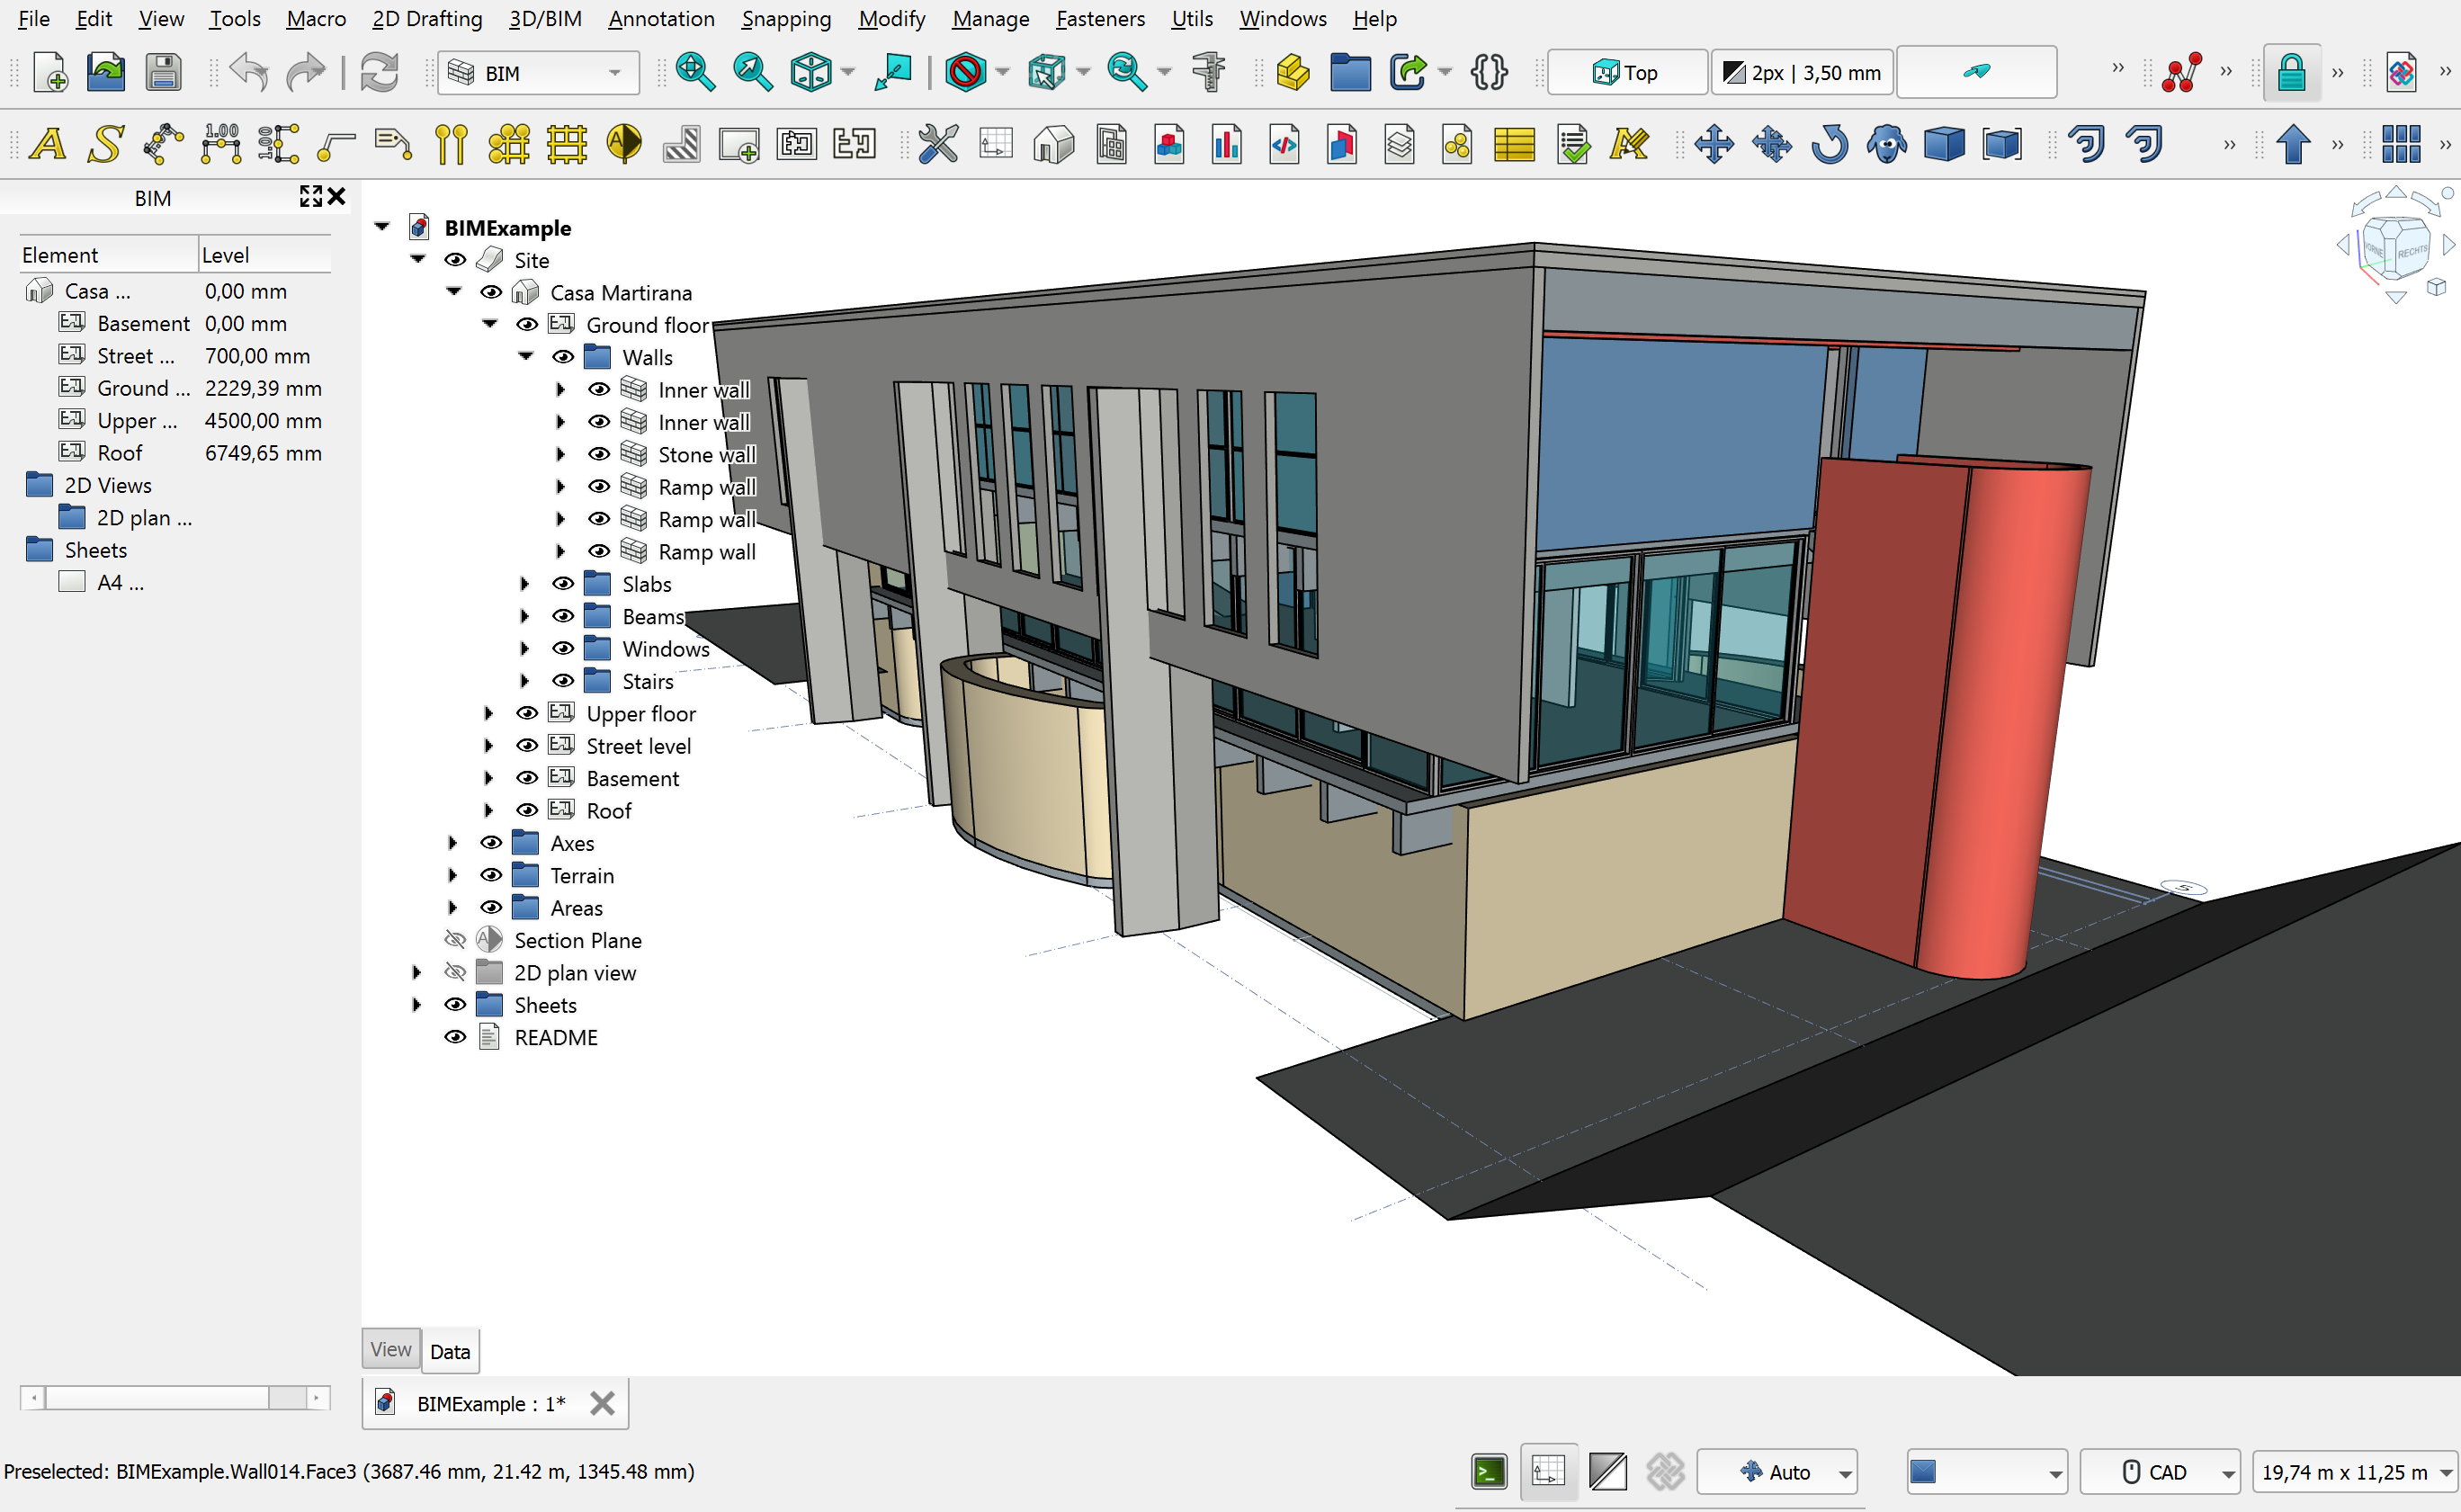
\includegraphics[width=0.8\textwidth]{img/cap2_interfaz.png}
	\caption{Vista de la interfaz de FreeCAD con área de trabajo}
\end{figure}

Aprende a moverte por FreeCAD. Conoce las áreas
principales de la interfaz y cómo navegar en 3D.

%% D. Búsqueda e Inserción de Activos Gráficos
%% Imagen insertada al inicio del capítulo

%% B. Actividades Teóricas
\section{Investigar y responder}
\faPencil

Investiga sobre la interfaz de FreeCAD y responde:
\begin{enumerate}
	\item ¿Cuáles son las áreas principales de la interfaz?
	\item ¿Qué función cumplen los workbenches o bancos de
	      trabajo?
	\item ¿Cómo se alternan entre vistas ortográficas y
	      perspectiva?
	\item ¿Qué atajos de teclado se usan para zoom, rotación
	      y desplazamiento?
	\item ¿Cómo personalizar la interfaz según tus necesidades?
	\item ¿Qué información muestra el árbol deCombo View?
	\item ¿Para qué sirve la barra de estado inferior?
	\item ¿Cómo cambiar entre diferentes workbenches?
\end{enumerate}

%% C. Actividades Prácticas
\section{Resolver los siguientes problemas}
\faWrench

Problemas para aplicar conocimientos:
\begin{enumerate}
	\item Abre FreeCAD y navega entre los diferentes
	      workbenches disponibles.
	\item Practica el zoom con la rueda del ratón y los
	      atajos de teclado.
	\item Realiza una rotación completa del espacio 3D
	      usando diferentes métodos.
	\item Cambia entre vista isométrica, frontal, lateral
	      y superior.
	\item Personaliza el tamaño y posición de los paneles
	      laterales.
	\item Guarda una configuración personalizada de
	      interfaz.
	\item Abre el archivo de ejemplo ``shaft.FCStd'' y
	      explora sus componentes en el árbol.
	\item Activa y desactiva la cuadrícula en el área de
	      trabajo.
	\item Configura las preferencias de visualización para
	      mejorar el rendimiento.
	\item Realiza una captura de pantalla con tu interfaz
	      personalizada y anota los cambios realizados.
\end{enumerate}